\begin{figure}[tbp]
  \centering
  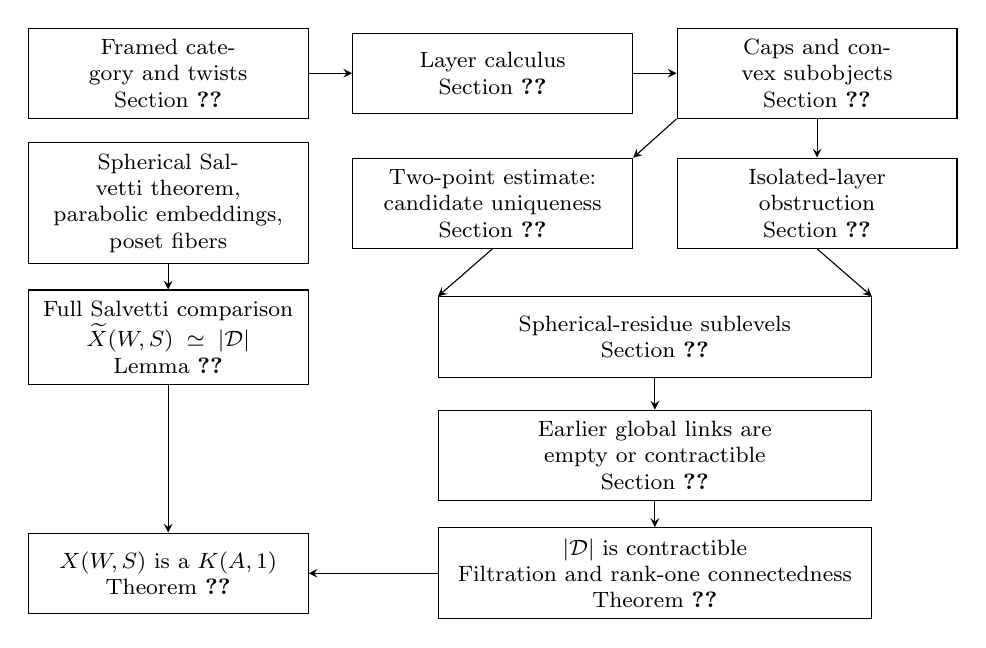
\begin{tikzpicture}[
      x=.01\linewidth,y=1cm,
      every node/.style={font=\footnotesize,align=center},
      result/.style={draw,thin,text width=.27\linewidth,
        minimum height=1.02cm,inner sep=4pt},
      wide/.style={result,text width=.43\linewidth},
      implication/.style={->,thin,>=stealth}
    ]
    \node[result] (category) at (0,0)
      {Framed category and twists\\Section~\ref{sec:category}};
    \node[result] (layers) at (34,0)
      {Layer calculus\\Section~\ref{sec:layers}};
    \node[result] (convexity) at (68,0)
      {Caps and convex subobjects\\Section~\ref{sec:height-data}};
    \node[result] (classical) at (0,-1.65)
      {Spherical Salvetti theorem,\\parabolic embeddings,\\poset fibers};
    \node[result] (two-point) at (34,-1.65)
      {Two-point estimate:\\candidate uniqueness\\Section~\ref{sec:two-point}};
    \node[result] (rigidity) at (68,-1.65)
      {Isolated-layer obstruction\\Section~\ref{sec:rigidity}};
    \node[result] (comparison) at (0,-3.35)
      {Full Salvetti comparison\\$\widetilde X(W,S)\simeq|\mathcal D|$\\
        Lemma~\ref{lem:salvetti-comparison}};
    \node[wide] (residues) at (51,-3.35)
      {Spherical-residue sublevels\\Section~\ref{sec:residues}};
    \node[wide] (links) at (51,-4.85)
      {Earlier global links are empty or contractible\\Section~\ref{sec:global}};
    \node[wide] (contractibility) at (51,-6.35)
      {$|\mathcal D|$ is contractible\\
        Filtration and rank-one connectedness\\
        Theorem~\ref{thm:deligne-contractible}};
    \node[result] (target) at (0,-6.35)
      {$X(W,S)$ is a $K(A,1)$\\Theorem~\ref{thm:main}};

    \draw[implication] (category) -- (layers);
    \draw[implication] (layers) -- (convexity);
    \draw[implication] (convexity.south west) -- (two-point.north east);
    \draw[implication] (convexity) -- (rigidity);
    \draw[implication] (two-point.south) -- (residues.north west);
    \draw[implication] (rigidity.south) -- (residues.north east);
    \draw[implication] (residues) -- (links);
    \draw[implication] (links) -- (contractibility);
    \draw[implication] (classical) -- (comparison);
    \draw[implication] (comparison) -- (target);
    \draw[implication] (contractibility) -- (target);
  \end{tikzpicture}
  \caption{The main dependencies.  The two algebraic estimates are proved
    before their use in the induction on spherical residues.  The classical
    comparison is independent of the height argument and transfers the
    resulting contraction to the full Salvetti universal cover.  Arrows
    display the main flow of the proof; the finite-type Coxeter and monoid
    inputs to the algebraic constructions are specified in the text.}
  \label{fig:dependencies}
\end{figure}
